\documentclass[main.tex]{subfiles}
\begin{document}
	
	In this section, we present the initial results of our implementation of the GRIN framework. The measurements presented here can only be considered preliminary, given the compiler needs further work to be comparable to systems like the Glasgow Haskell Compiler or the Idris compiler~\cite{idris}. Nevertheless, these statistics are still relevant, since they provide valuable information about the effectiveness of the optimizer.
	
	%TODO: compilation process to different section
	\subsection{Setup}
	
	%TODO: include code of Length
	The measurements were taken using the Idris front end and LLVM back end of the compiler. Each test program --- besides ``Length" --- was taken from the book \textit{Type-driven development with Idris}~\cite{tdd-idris} by Edwin Brady. These are small Idris programs demonstrating a certain aspect of the language. 
	
	\subsubsection{Front end}
	
	The front end uses the bytecode produced by the Idris compiler to generate the GRIN intermediate representation. The code generation itself is really simple, the difficult part of refining the original program is handled by the optimizer. 
	
	\subsubsection{Optimizer}
	
	The optimization pipeline consists of three stages. In the first stage, the optimizer iteratively runs the so-called \textit{regular optimizations}. These are the program transformations described in Urban Boquist's PhD thesis~\cite{boquist-phd}. A given pipeline of these transformations are run until the code reaches a fixed-point, and cannot be optimized any further. This set of transformation are not formally proven to be confluent, so theoretically different pipelines can result in different fixed-points\footnote{Although, experiments suggest that these transformations \textit{are} confluent}. Furthermore, some of these transformations can work against each other, so a fixed-point may not always exist. In this case, the pipeline can be caught in a loop, where the program returns to the same state over and over again. Fortunately, these loops can be detected, and the transformation pipeline can be terminated. 
	
	%TODO: use process diagram template from TDK
	\vspace{-0.6cm}
	\begin{figure}[H]
		\centering
		\begin{adjustbox}{scale = 1.3}
			\tikzset{every loop/.style={-{Stealth[scale=1.5]}}}
			
			%\hspace{-1cm}
			\begin{tikzpicture}[ node distance = 1.5cm and 3cm
												 , on grid 
												 , loop/.append style={-triangle 60}
												 ]
			
			\node [draw=black] (cg)    									{Code gen.};
			\node [draw=black] (ro1) [right =of cg]  {Regular Opts.};
			\node [draw=black] (dde) [right =2.5cm of ro1]  {DDE};
			\node [draw=black] (ro2) [right =2.5cm of dde]  {Regular Opts.};
			
			\path[-{Stealth[scale=1.5]}] 
			(cg) edge [] (ro1)
			(ro1) edge [loop] (ro1)
			(ro1) edge [] (dde)
			(dde) edge [] (ro2)
			(ro2) edge [loop] (ro2);
			
			
			\end{tikzpicture}
		\end{adjustbox}
		\caption{The optimization stages}
		\label{fig:-measurement-pipeline}
	\end{figure}

	Following that, in the second stage, the optimizer runs the \textit{dead data elimination pass}. This pass can be quite demanding on both the memory usage and the execution time due to the several data-flow analyses the transformation requires. Also, it is a rather specific transformation, which means, running it multiple times might not improve the code any further. As a consequence, the dead data elimination pass is executed only a single time during the entire optimization process. Since the dead data elimination pass can enable other optimizations, the optimizer runs the regular optimizations a second time right after the DDE pass.
	
	\subsubsection{Back end}
	
	%TODO: optimization levels?
	After the optimization process, the optimized GRIN code is passed onto the back end, which then generates an executable using the LLVM compiler framework. The input of the back end consists of the optimized GRIN code, the primitive operations of Idris and a minimal runtime (the latter two are both implemented in C). Currently, the runtime is only responsible for allocating heap memory for the program, and at this point it does not include a garbage collector.
	
	The first task of the back end is to compile the GRIN code into LLVM IR code which is then optimized further by the LLVM Modular Optimizer~\cite{opt}. After that, the optimized LLVM code is compiled into an object file by the LLVM Static Compiler~\cite{llc}. Finally, Clang links together the object file with the C-implemented primitive operations and the runtime, and generates an executable binary.
	
	\subsection{Measured metrics}
	
	% DONE
	%- idris FR, LLVM BE
	%- small programs from TDD
	%- simple code generation
	%- no GC
	%- pipeline setup
	
	% TODO
	%- cant compare to IC
	%- compile & runtime stats for GRIN IR
	%- runtime stats for binary
	
	
	\begin{figure}
		\hspace{-0.5cm}
		\renewcommand{\figurename}{Diagram}
		\caption{Length - GRIN statistics}
		\label{diagram:length-stats}
		\addtocounter{figure}{-1}
		\begin{minipage}{0.5\textwidth}
			\subcaption{Runtime}
			\resizebox{\width}{7cm}{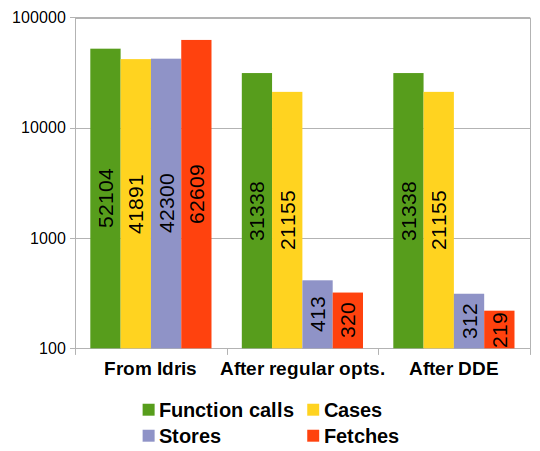
\includegraphics[scale=0.55]{length-runtime.png}}
		\end{minipage}
		\begin{minipage}{0.5\textwidth}
			\subcaption{Compile time}
			\resizebox{\width}{7cm}{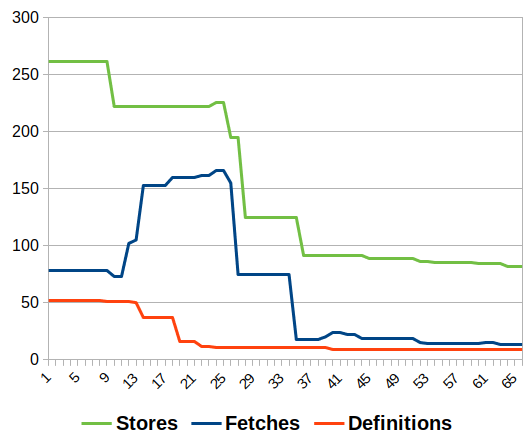
\includegraphics[scale=0.55]{length-compile-time.png}}
		\end{minipage}
	\end{figure}

	\begin{figure}
		\hspace{-0.5cm}
		\renewcommand{\figurename}{Diagram}
		\caption{Exact length - GRIN statistics}
		\label{diagram:exact-length-stats}
		\addtocounter{figure}{-1}
		\begin{minipage}{0.5\textwidth}
			\subcaption{Runtime}
			\resizebox{\width}{7cm}{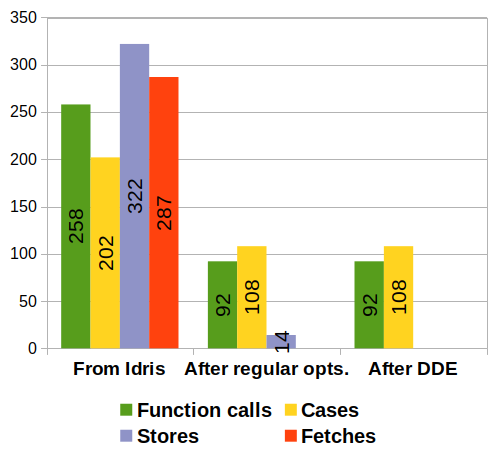
\includegraphics[scale=0.55]{exact-length-runtime.png}}
		\end{minipage}
		\begin{minipage}{0.5\textwidth}
			\subcaption{Compile time}
			\resizebox{\width}{7cm}{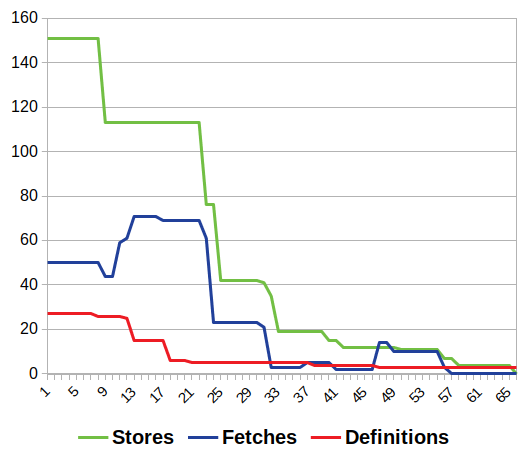
\includegraphics[scale=0.55]{exact-length-compile-time.png}}
		\end{minipage}
	\end{figure}
	
	\begin{figure}
		\hspace{-0.5cm}
		\renewcommand{\figurename}{Diagram}
		\caption{Type level functions - GRIN statistics}
		\label{diagram:tyfuns-stats}
		\addtocounter{figure}{-1}
		\begin{minipage}{0.5\textwidth}
			\subcaption{Runtime}
			\resizebox{\width}{7cm}{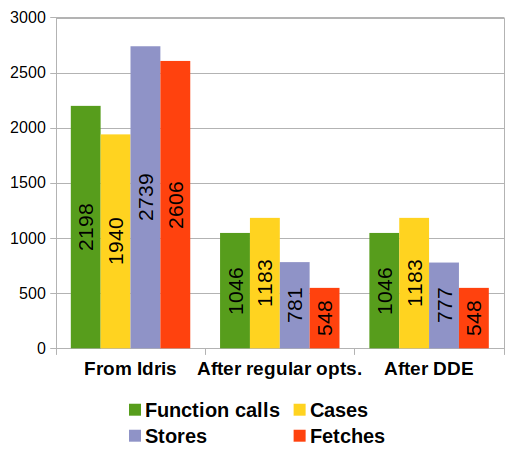
\includegraphics[scale=0.55]{tyfuns-runtime.png}}
		\end{minipage}
		\begin{minipage}{0.5\textwidth}
			\subcaption{Compile time}
			\resizebox{\width}{7cm}{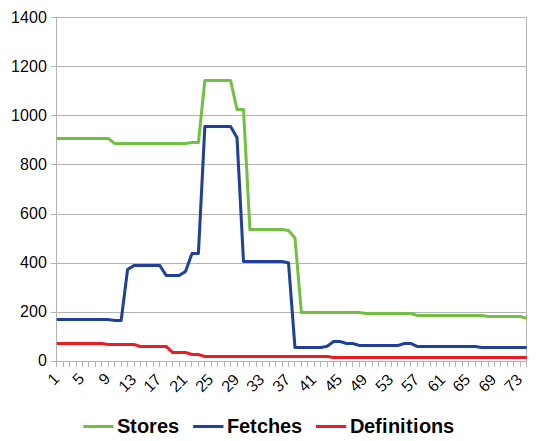
\includegraphics[scale=0.55]{tyfuns-compile-time.png}}
		\end{minipage}
	\end{figure}
	
	\begin{figure}
		\hspace{-0.5cm}
		\renewcommand{\figurename}{Diagram}
		\caption{Reverse - GRIN statistics}
		\label{diagram:reverse-stats}
		\addtocounter{figure}{-1}
		\begin{minipage}{0.5\textwidth}
			\subcaption{Runtime}
			\label{diagram:reverse-stats-a}
			\resizebox{\width}{7cm}{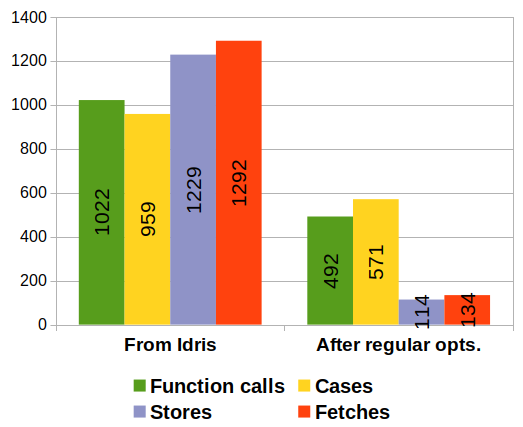
\includegraphics[scale=0.55]{reverse-runtime.png}}
		\end{minipage}
		\begin{minipage}{0.5\textwidth}
			\subcaption{Compile time}
			\label{diagram:reverse-stats-b}
			\resizebox{\width}{7cm}{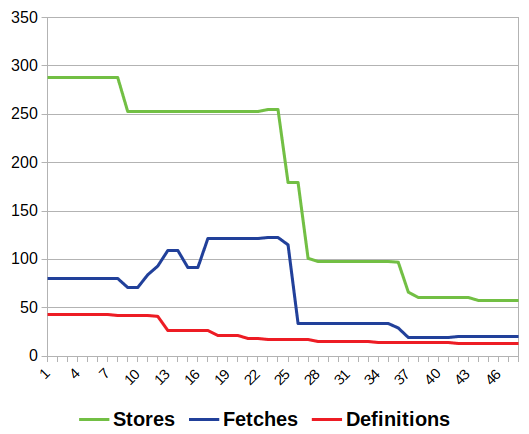
\includegraphics[scale=0.55]{reverse-compile-time.png}}
		\end{minipage}
	\end{figure}
	
	\begin{center}
		\begin{minipage}{0.6\linewidth}
			\captionof{table}{Length - binary statistics}
			\label{table:length-binary-results}
			\begin{tcolorbox}[tab2,tabularx={l||r|r|r|r}]
				Stage                 & Size  & Instructions & Stores & Loads      \\
				\hline\hline
				\pilcode{normal-O0}   & 23928 & 769588 & 212567 & 233305 \\\hline
				\pilcode{normal-O3}   & 23928 & 550065 & 160252 & 170202 \\\hline
				\pilcode{regular-opt} & 19832 & 257397 & 14848  & 45499  \\\hline
				\pilcode{dde-O0}      & 15736 & 256062 & 14243  & 45083  \\\hline
				\pilcode{dde-O3}      & 15736 & 284970 & 33929  & 54555  \\
			\end{tcolorbox}	
		\end{minipage}
	\end{center}
	
	\begin{center}
		\begin{minipage}{0.58\linewidth}
			\captionof{table}{Exact length - binary statistics}
			\label{table:exact-length-binary-results}
			\begin{tcolorbox}[tab2,tabularx={l||r|r|r|r}]
				Stage                 & Size  & Instructions & Stores & Loads      \\
				\hline\hline
				\pilcode{normal-O0}   & 18800 & 188469 & 14852 & 46566 \\\hline
				\pilcode{normal-O3}   & 14704 & 187380 & 14621 & 46233 \\\hline
				\pilcode{regular-opt} & 10608 & 183560 & 13462 & 45214 \\\hline
				\pilcode{dde-O0}      & 10608 & 183413 & 13431 & 45189 \\\hline
				\pilcode{dde-O3}      & 10608 & 183322 & 13430 & 44226 \\
			\end{tcolorbox}	
		\end{minipage}
	\end{center}
	
	\begin{center}
		\begin{minipage}{0.58\linewidth}
			\captionof{table}{Type level functions - binary statistics}
			\label{table:tyfuns-binary-results}
			\begin{tcolorbox}[tab2,tabularx={l||r|r|r|r}]
				Stage                 & Size  & Instructions & Stores & Loads      \\
				\hline\hline
				\pilcode{normal-O0}   & 65128 & 383012 & 49191 & 86754 \\\hline
				\pilcode{normal-O3}   & 69224 & 377165 & 47556 & 84156 \\\hline
				\pilcode{regular-opt} & 36456 & 312122 & 34340 & 71162 \\\hline
				\pilcode{dde-O0}      & 32360 & 312075 & 34331 & 70530 \\\hline
				\pilcode{dde-O3}      & 28264 & 309822 & 33943 & 70386 \\
			\end{tcolorbox}	
		\end{minipage}
	\end{center}
	
	\begin{center}
		\begin{minipage}{0.62\linewidth}
			\captionof{table}{Reverse - binary statistics}
			\label{table:reverse-binary-results}
			\begin{tcolorbox}[tab2,tabularx={l||r|r|r|r}]
				Stage                 & Size  & Instructions & Stores & Loads      \\
				\hline\hline
				\pilcode{normal-O0}      & 27112 & 240983 & 25018 & 58253 \\\hline
				\pilcode{normal-O3}      & 31208 & 236570 & 23808 & 56617 \\\hline
				\pilcode{regular-opt-O0} & 14824 & 222085 & 19757 & 53125 \\\hline
				\pilcode{regular-opt-O3} & 14824 & 220837 & 19599 & 52827 \\
			\end{tcolorbox}	
		\end{minipage}
	\end{center}

\end{document}